\documentclass[12pt,fleqn,answers]{exam}
\usepackage{pifont}
\usepackage{dingbat}
\usepackage{amsmath,amssymb}
\usepackage{epsfig}
\usepackage{graphicx}
\usepackage[]{hyperref}
\usepackage{geometry}
\geometry{letterpaper, margin=0.75in}
\addpoints
\boxedpoints
\pointsinmargin
\pointname{pts}

\usepackage[activate={true,nocompatibility},final,tracking=true,kerning=true,factor=1100,stretch=10,shrink=10]{microtype}
\usepackage[american]{babel}
%\usepackage[T1]{fontenc}
\usepackage{fourier}
\usepackage{isomath}
\usepackage{upgreek,amsmath}
\usepackage{amssymb}

\newcommand{\dotprod}{\, {\scriptzcriptztyle
    \stackrel{\bullet}{{}}}\,}

\newcommand{\reals}{\mathbf{R}}
\newcommand{\lub}{\mathrm{lub}} 
\newcommand{\glb}{\mathrm{glb}} 
\newcommand{\complex}{\mathbf{C}}
\newcommand{\dom}{\mbox{dom}}
\newcommand{\cover}{{\mathcal C}}
\newcommand{\integers}{\mathbf{Z}}
\newcommand{\vi}{\, \mathbf{i}}
\newcommand{\vj}{\, \mathbf{j}}
\newcommand{\vk}{\, \mathbf{k}}
\newcommand{\bi}{\, \mathbf{i}}
\newcommand{\bj}{\, \mathbf{j}}
\newcommand{\bk}{\, \mathbf{k}}
\DeclareMathOperator{\Arg}{\mathrm{Arg}}
\DeclareMathOperator{\Ln}{\mathrm{Ln}}
\newcommand{\imag}{\, \mathrm{i}}
\newcommand{\range}{\mathrm{range}}
\newcommand{\ball}{\mathrm{ball}}
\newcommand{\LP}{\mathrm{LP}}

\usepackage{graphicx}
\newcommand\AM{{\sc am}}
\newcommand\PM{{\sc pm}}
     
\newcommand{\quiz}{0}
\newcommand{\term}{Fall}
\newcommand{\due}{Friday 25 August  at 11:59 \PM}
\begin{document}
\large
\vspace{0.1in}
\noindent\makebox[3.0truein][l]{{\bf MATH 202}}
{\bf Name:} \hrulefill \\
\noindent \makebox[3.0truein][l]{\bf Calculus Practice I, \term \/ \the\year}
%{\bf Row:}\hrulefill\
\vspace{0.1in}

\noindent Here is an opportunity for you to maintain your calculus skills
over the summer. If you complete these problems,
digitize your work, and submit your work to Canvas, I will send you my
solutions. If you need some help with these questions, 
email me with your questions (\href{mailto:willisb@unk.edu}{willisb@unk.edu})

Completing this work is optional, and it does not 
enter into your class grade in any way--this work is 
 not a bonus, extra credit, or anything like that.

\begin{questions}


\question Find an equation of the tangent line to the 
curve $y = \sqrt{x^2+1}$ at the point \mbox{$(x=1, y=\sqrt{2})$.}
\begin{solution}[2.5in]

To find an equation of a line we need to know (a) its slope and (b) a point on the
line.  We're given a point on the line, so our main task is to find the slope of the 
tangent line. To do that we need to first find a formula for \(\displaystyle
\frac{\mathrm{d} y}{\mathrm{d} x} \) and second we need to evaluate \(\displaystyle
\frac{\mathrm{d} y}{\mathrm{d} x} \) when $x=1$. The chain rule tell us that
\begin{equation}
    \frac{\mathrm{d} y}{\mathrm{d} x} = \frac{1}{2} \times 2 x (x^2+1)^{-1/2}
      = x (x^2+1)^{-1/2}.
\end{equation}
And pasting in $x \to 1$, we have
\begin{equation}
    \left . \frac{\mathrm{d} y}{\mathrm{d} x} \right |_{x=1}=  
    \left .  x (x^2+1)^{-1/2} \right |_{x=1} =
    \frac{1}{\sqrt{2}}.
\end{equation}
An equation of the given tangent line is
\begin{equation}
  y - \sqrt{2} = \frac{1}{\sqrt{2}} (x-1)
\end{equation}

Traditionally, we would simplify \(\frac{1}{\sqrt{2}}\)
to \(\frac{\sqrt{2}}{2}\) and add $\sqrt{2}$ to solve for $y$. Doing so results in
\begin{equation}
  y= \frac{\sqrt{2}}{2} (x+1).
\end{equation}
Arguably, $ y= \frac{\sqrt{2}}{2} (x+1)$ is more simple than is $y - \sqrt{2} = \frac{\sqrt{2}}{2} (x-1)$.
But in this context, I don't see much of an advantage to doing this. In the first formula $y - \sqrt{2} = \frac{1}{\sqrt{2}} (x-1)$
it's clear that $(x=1, y=\sqrt{2})$ is a point on the line.  

In short, all the answers
\begin{align*}
  &y - \sqrt{2} = \frac{1}{\sqrt{2}} (x-1),\\
  &y =  \frac{1}{\sqrt{2}} (x+1),\\
  &y =\frac{\sqrt{2}}{2} (x+1),
 \end{align*}
 are OK answers to the question ``Find an equation of the tangent line.'' Semantically, all these answers are equivalent and
 each of them are simplified according to our class standard: (from the class FAQ)
 
 \textbf{Question} Is this OK, or do I need to simplify it?

\textbf{Answer} Maybe. Giving guidelines on what it means to 
  simplified is tough. But if you  (a) do all rational arithmetic (b) combine
  all like terms, (c) simplify all ``famous'' values of functions, 
  for example $\cos(0)=1$ and $\sqrt{81} = 9$, and (d) make an effort
  to simplify all vanishing subexpressions to zero (for example, 
  $\frac{1}{\sqrt{2}} - \frac{\sqrt{2}}{2}$ simplifies to zero), you'll be OK.

\quad Instead of worrying so much about simplifying expressions according to a murky and 
unpublished rule, let's shift our
main attention on to learning to use various tools to check our work. For this question, a graph is a good way
to check that the line and the curve are tangent.   Let's ask Desmos to draw 
graphs of both $y=\sqrt{1+x^2}$ and $y - \sqrt{2} = \frac{1}{\sqrt{2}} (x-1)$. Does the line and the curve
appear to be tangent?  Sure.

    \centering
    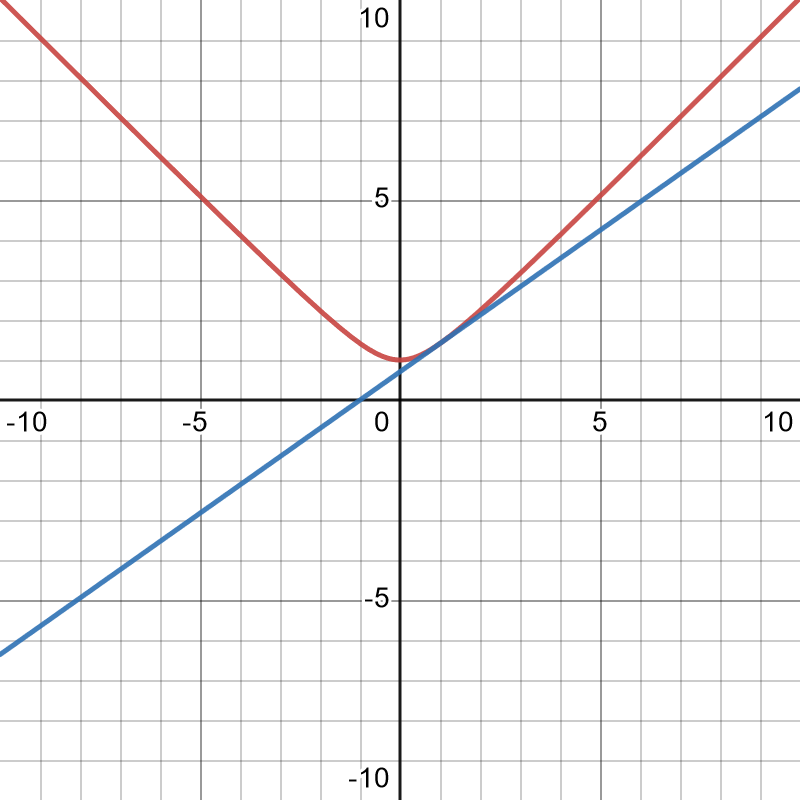
\includegraphics[scale=0.2]{desmos-graph(44).png}

The picture is fairly convincing--we have a (not the) correct answer.


\end{solution}

\newpage

\question Find each antiderivative.

\begin{parts}
    
    \part $\int x^2 - x - 2 \, \mathrm{d} x $
    \begin{solution}[2.5in]
  
    \begin{equation}
      \int x^2 - x - 2 \, \mathrm{d} x = \frac{1}{3} x^3 - \frac{1}{2} x^2 - 2 x.
      \end{equation}
    Some teachers will insist on the $+c$.  I say let's just  remember that all 
    antiderivatives are undetermined up to an additive constant.
   
    \quad Notice that the $+c$ rule is a problem if the variable name is $c$. Should we add $+c$ to
    \begin{equation}
      \int c^2 - c - 2 \, \mathrm{d} c = \frac{1}{3} c^3 - \frac{1}{2} c^2 - 2 c?
      \end{equation}
     Unless we want a wrong answer, no we should not.
    \end{solution}

    \part $\int (x-1)(x+2) \, \mathrm{d} x $
    \begin{solution}[2.5in] This one is a freebie.  Expanding the integrand, this problem is the same as the previous problem.
    
    \quad It's tempting, I know, but do not make the \textbf{error} of thinking that that the anti derivative of a product is 
    the product of the anti derivatives. That is \text{do not do}
    \begin{equation}
      \int (x-1)(x+2) \, \mathrm{d} x = \frac{1}{2} (x-1)^2 \times \frac{1}{2} (x+2)^2
    \end{equation}
    We should practice the good habit of checking anti derivatives by differentiating. Doing so we have
    \begin{align*}
      \frac{\mathrm{d}}{\mathrm{d} x} \left(\frac{1}{2} (x-1)^2 \times \frac{1}{2} (x+2)^2 \right)
          &= \frac{\left( x-1\right) \, {{\left( x+2\right) }^{2}}}{2}+\frac{{{\left( x-1\right) }^{2}}\, \left( x+2\right) }{2},\\
          &= \frac{\left( x-1\right) \, \left( x+2\right) \, \left( 2 x+1\right) }{2}, \\
          &= {{x}^{3}}+\frac{3 {{x}^{2}}}{2}-\frac{3 x}{2}-1.
   \end{align*}
   This is not equivalent to the integrand $(x-1)(x+2) $, so our work is \textbf{wrong}.
        \end{solution}



    \part $\int \frac{1+x^2}{x^2} \, \mathrm{d} x$

\begin{solution} On any interval on that does not contain zero, we have
\begin{align*}
\int \frac{1+x^2}{x^2} \, \mathrm{d} x &= \int x^{-2} + 1 , \mathrm{d} x, \\
                                                          &=- \frac{1}{x} + x.
\end{align*}
If you worked this problem with a first step something like
\begin{equation}
\int \frac{1+x^2}{x^2} \, \mathrm{d} x = \frac{x^2 \int 1+x^2 \, \mathrm{d} x - (1+x^2) \int x^2 \, \mathrm{d} x}
 {\left(\int x^2 \, \mathrm{d} x\right)^2}
\end{equation}
let's make this the very last time you make this mistake.

\end{solution}
\end{parts}

\newpage

\question Find each definite integral.


\begin{parts}
    
    \part $\int_1^2 x^2 - x - 2 \, \mathrm{d} x $
    \begin{solution}[2.5in]
    In the previous question, we found the antiderivative; so all we need to do is
    \begin{equation}
    \int_1^2 x^2 - x - 2 \, \mathrm{d} x = \left . \frac{1}{3} x^3 - \frac{1}{2} x^2 - 2 x \right |_{x=1}^{x=2}
     = - \frac{7}{6}.
    \end{equation}
    Graphically, we can tell that this definite integral is negative. Why? The graph of the integrand is entirely below
    the x-axis, that's why. Here is a graph of the integrand
    
    \quad \quad \quad 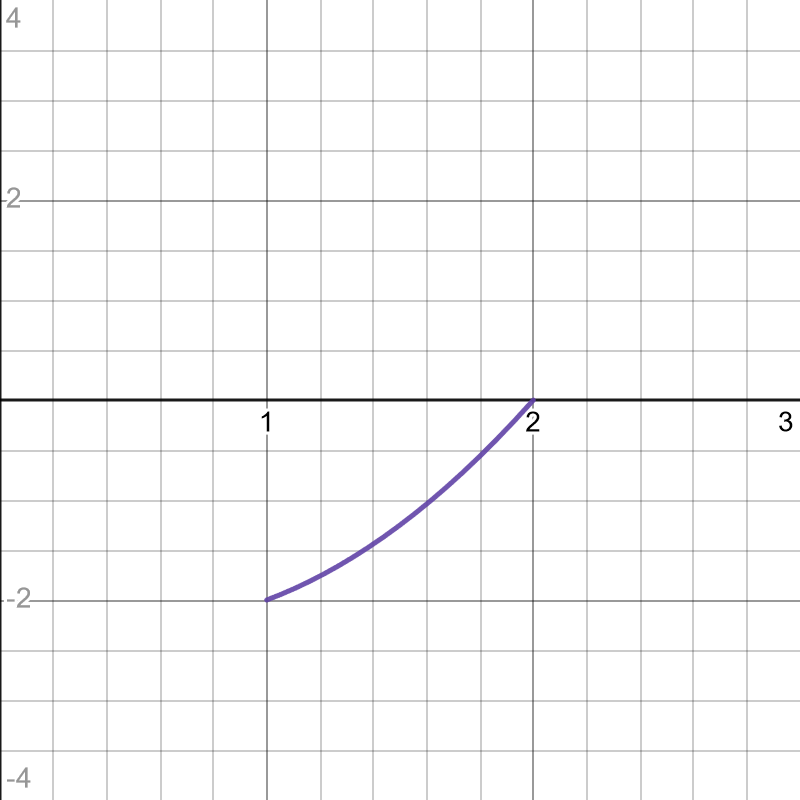
\includegraphics[scale=0.2]{desmos-graph(45).png}
    
    Actually, the graph of the integrand on the interval $[1,2]$ is pretty well approximated by a line segment joining 
    $(x=1,y=-2)$ and  $(x=2,y=0)$. Doing so, we see that  $ \int_1^2 x^2 - x - 2 \, \mathrm{d} x $ is pretty close
    to the negative of the area of a triangle with base one and height two. So $ \int_1^2 x^2 - x - 2 \, \mathrm{d} x \approx -1$. And I'd say that $- \frac{7}{6} \approx -1$.
    

    \end{solution}

    \part $\int_1^2 (x-1)(x+2) \, \mathrm{d} x $
    \begin{solution}[2.5in]
    Expanding the integrand, we see that we've done this problem before.
    \end{solution}



    \part $\int_1^4 \frac{1+x^2}{x^2} \, \mathrm{d} x$
    
    \begin{solution} We have
    \begin{align*}
    \int_1^4 \frac{1+x^2}{x^2} \, \mathrm{d} x &= \left. \left(- \frac{1}{x} + x \right) \right |_{x=1}^{x=4}, \\
                                                                      &= \frac{15}{4}.
    \end{align*}
    
    \end{solution}


\end{parts}

\newpage

\question For each function $F$, find the solution set of $F^\prime(x)  = 0$.  

\begin{parts}

    \part $F(x) = x^2+x+3$
    \begin{solution}[2.5in] We need to solve
    \begin{equation}
      \left[2x + 1 = 0 \right] = \left[x=-1/2 \right].
    \end{equation}
    \end{solution}

    \part $F(x) = (x-3)(x^2+3)$
    \begin{solution}[2.5in] Using the product rule, we have $F^\prime(x) = 3 {{x}^{2}}-6 x+3$. So we
    need to solve
     \begin{align*}
      \left[3 {{x}^{2}}-6 x+3 \right] &= \left[  3 {{\left( x-1\right) }^{2}} \right] & \mbox{(factor)} \\
                                                   &= \left[x=1\right].
    \end{align*}
    \end{solution}

    \part $F(x) = 2 x +  \frac{x}{x-2}$
    \begin{solution}[2.5in] We have
    \begin{equation} 
      F^\prime(x) = \frac{2 \left( x-3\right) \, \left( x-1\right) }{{{\left( x-2\right) }^{2}}}.
    \end{equation}
    We have
    \begin{align*}
        \left[ F^\prime(x) = 0 \right] &=
           \left[ \frac{2 \left( x-3\right) \, \left( x-1\right) }{{{\left( x-2\right) }^{2}}} = 0 \right], \\
           &= \left[ 0 = (x-3)(x-1), x-2 \neq 0 \right], \\
           &= \left[x=3, x=2\right].
    \end{align*}
    \end{solution}

    \part $F(x) = \cos(x) \sin(x)$
    \begin{solution}[2.5in] I think this problem is easier if we 
      use the indentity $\cos(x) \sin(x) = \frac{1}{2} \sin(2 x)$. So
      \begin{align*}
        \left[ F^\prime(x) = 0 \right] &= \left[\cos(2 x) = 0 \right], \\
            &= \left[ 2 x = \uppi (k  - \frac{1}{2}), k \in \mathbf{Z} \right], \\
            &= \left[x = \frac{\uppi}{2} \left (k  - \frac{1}{2} \right), 
            k \in \mathbf{Z} \right],
      \end{align*}
    \end{solution}


\end{parts}

\newpage

\question Find the value of each limit.

\begin{parts}

\part $\displaystyle \lim_{x \to 4} \frac{\cos(x)+1}{x-3}$
\begin{solution}[2.5in] The function is continuous at 4, so we can use DS (direct substitution); we have
\begin{equation}
 \lim_{x \to 4} \frac{\cos(x)+1}{x-3} = \cos(4)+1.
\end{equation}
If somebody wants a decimal approximation to $\cos(4)+1$ to any number of digits, they can do that.
    
\end{solution}

\part $\displaystyle \lim_{x \to 4} \frac{{{x}^{2}}-2 x-3}{x-3}$
\begin{solution}[2.5in] Again, the function is continuous at 4, so let's use DS; we have
\begin{equation}
  \lim_{x \to 4} \frac{{{x}^{2}}-2 x-3}{x-3} = 4^2-2 \times 4 - 3 = 5.
\end{equation}
    
\end{solution}

\part $\displaystyle \lim_{x \to \infty} \frac{5 x^2 + x+1}{7 x^2 + 107}$

\begin{solution}
Toward $\infty$, the dominate term of the numerator is $5 x^2$;
and the dominate term of the denominator is $7 x^2$. So
\begin{align*}
  \lim_{x \to \infty} \frac{5 x^2 + x+1}{7 x^2 + 107}
     = \lim_{x \to \infty} \frac{5 x^2}{7 x^2} = \frac{5}{7}.
\end{align*}
  
\end{solution}
\end{parts}
\end{questions}




\end{document}